\documentclass[border=6pt, multi, tikz]{standalone}
\usetikzlibrary{positioning, arrows.meta, calc, fit, backgrounds,
                 decorations.pathreplacing}
\usepackage{amsmath, amssymb}

% ── Colour palette ──
\definecolor{liftcol}{RGB}{245,155,50}
\definecolor{senscol}{RGB}{70,170,70}
\definecolor{mortedge}{RGB}{31,119,180}
\definecolor{knnedge}{RGB}{140,90,180}
\definecolor{gridln}{RGB}{195,195,195}
\definecolor{gridfl}{RGB}{244,244,244}
\definecolor{hilight}{RGB}{255,230,180}
\definecolor{edgecol}{RGB}{100,100,100}

\begin{document}
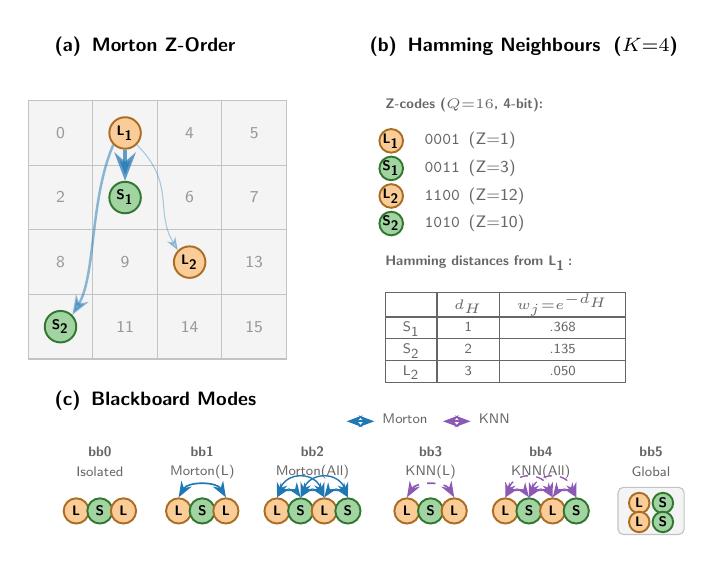
\begin{tikzpicture}[
    >=Stealth,
    % Grid cell
    gc/.style={draw=gridln, minimum size=0.82cm, inner sep=0pt,
               font=\sffamily\fontsize{6}{7}\selectfont\color{black!40},
               fill=gridfl, anchor=center},
    % Agent circle
    ag/.style={circle, draw, line width=0.7pt, minimum size=0.40cm,
               inner sep=0pt, font=\sffamily\fontsize{5.5}{6}\selectfont\bfseries},
    lift/.style={ag, fill=liftcol!50, draw=liftcol!70!black},
    sens/.style={ag, fill=senscol!50, draw=senscol!70!black},
    % Titles
    ptitle/.style={font=\sffamily\fontsize{7.5}{9}\selectfont\bfseries},
    stxt/.style={font=\sffamily\fontsize{5.5}{6.5}\selectfont, text=black!60},
    mtxt/.style={font=\sffamily\fontsize{5}{6}\selectfont\itshape, text=black!50},
]

% ══════════════════════════════════════════════════════════════
% (a)  Morton Z-Order  ·  4×4 example
% ══════════════════════════════════════════════════════════════
\node[ptitle, anchor=south west] at (-0.2, 3.65)
    {(a)\enspace Morton Z-Order};

% ── Grid cells  (row, col) → Z-index ──
\foreach \r/\c/\z in {
    0/0/0,  0/1/1,  0/2/4,  0/3/5,
    1/0/2,  1/1/3,  1/2/6,  1/3/7,
    2/0/8,  2/1/9,  2/2/12, 2/3/13,
    3/0/10, 3/1/11, 3/2/14, 3/3/15}
{   \node[gc] (c\r\c) at (\c*0.82, 2.8-\r*0.82) {\z}; }

% ── Z-curve (thin, background) ──
\begin{scope}[on background layer]
\draw[edgecol!30, line width=0.6pt,
      dash pattern=on 2.5pt off 1.5pt,
      rounded corners=0.6pt]
    (c00.center) -- (c01.center) -- (c10.center) -- (c11.center)
    -- (c02.center) -- (c03.center) -- (c12.center) -- (c13.center)
    -- (c20.center) -- (c21.center) -- (c30.center) -- (c31.center)
    -- (c22.center) -- (c23.center) -- (c32.center) -- (c33.center);
\end{scope}

% ── Highlight L₁'s Hamming neighbours ──
\begin{scope}[on background layer]
\node[gc, fill=hilight] at (c01.center) {1};   % L₁
\node[gc, fill=hilight!60] at (c11.center) {3}; % S₁ (d=1)
\node[gc, fill=hilight!30] at (c30.center) {10}; % S₂ (d=2)
\end{scope}

% ── Agents ──
\node[lift] (aL1) at (c01.center) {L\textsubscript{1}};
\node[sens] (aS1) at (c11.center) {S\textsubscript{1}};
\node[lift] (aL2) at (c22.center) {L\textsubscript{2}};
\node[sens] (aS2) at (c30.center) {S\textsubscript{2}};

% ── Adjacency edges from L₁  (width ∝ attention weight) ──
\draw[mortedge, line width=1.6pt, opacity=0.7, ->, >=Stealth]
    (aL1.south) -- (aS1.north);  % d_H=1, w=.368
\draw[mortedge, line width=0.9pt, opacity=0.5, ->, >=Stealth]
    (aL1.south west) .. controls +(-0.3,-0.7) and +(0.3,0.5) .. (aS2.north east);
\draw[mortedge, line width=0.4pt, opacity=0.35, ->, >=Stealth]
    (aL1.south east) .. controls +(0.5,-0.5) and +(-0.3,0.5) .. (aL2.north west);

% ══════════════════════════════════════════════════════════════
% (b)  Hamming Neighbour Selection  (K=4)
% ══════════════════════════════════════════════════════════════
\node[ptitle, anchor=south west] at (3.8, 3.65)
    {(b)\enspace Hamming Neighbours\; ($K{=}4$)};

\node[stxt, anchor=west, font=\sffamily\fontsize{5.5}{6.5}\selectfont\bfseries] at (4.0, 3.15)
    {Z-codes ($Q{=}16$, 4-bit):};

% Agent codes table
\node[lift, minimum size=0.30cm] at (4.2, 2.70) {\tiny L\textsubscript{1}};
\node[stxt, anchor=west, font=\sffamily\fontsize{6}{7}\selectfont]
    at (4.5, 2.70) {\texttt{0001}\enspace(Z{=}1)};

\node[sens, minimum size=0.30cm] at (4.2, 2.35) {\tiny S\textsubscript{1}};
\node[stxt, anchor=west, font=\sffamily\fontsize{6}{7}\selectfont]
    at (4.5, 2.35) {\texttt{00\textbf{1}1}\enspace(Z{=}3)};

\node[lift, minimum size=0.30cm] at (4.2, 2.00) {\tiny L\textsubscript{2}};
\node[stxt, anchor=west, font=\sffamily\fontsize{6}{7}\selectfont]
    at (4.5, 2.00) {\texttt{\textbf{11}0\textbf{0}}\enspace(Z{=}12)};

\node[sens, minimum size=0.30cm] at (4.2, 1.65) {\tiny S\textsubscript{2}};
\node[stxt, anchor=west, font=\sffamily\fontsize{6}{7}\selectfont]
    at (4.5, 1.65) {\texttt{\textbf{1}0\textbf{1}0}\enspace(Z{=}10)};

% Distance table
\node[stxt, anchor=west, font=\sffamily\fontsize{5.5}{6.5}\selectfont\bfseries] at (4.0, 1.15)
    {Hamming distances from L\textsubscript{1}\,:};

\node[stxt, anchor=north west] at (4.0, 0.90) {%
    \renewcommand{\arraystretch}{1.15}%
    \begin{tabular}{|l|c|c|}
    \hline
    & $d_H$ & $w_j{=}e^{-d_H}$ \\
    \hline
    S\textsubscript{1} & 1 & .368 \\
    \hline
    S\textsubscript{2} & 2 & .135 \\
    \hline
    L\textsubscript{2} & 3 & .050 \\
    \hline
    \end{tabular}};

% ══════════════════════════════════════════════════════════════
% (c)  Blackboard Modes  ·  bb0 – bb5
% ══════════════════════════════════════════════════════════════
\node[ptitle, anchor=south west] at (-0.2, -0.85)
    {(c)\enspace Blackboard Modes};

% --- helper y-levels ---
\def\bbLabelY{-1.25}
\def\bbSubY{-1.50}
\def\bbAgentY{-2.00}

% ── bb0  Isolated ──
\def\bx{0.5}
\node[stxt, font=\sffamily\fontsize{5.5}{6.5}\selectfont\bfseries]
    at (\bx, \bbLabelY) {bb0};
\node[stxt] at (\bx, \bbSubY) {Isolated};
\node[lift, minimum size=0.32cm] at (\bx-0.3, \bbAgentY) {\tiny L};
\node[sens, minimum size=0.32cm] at (\bx,     \bbAgentY) {\tiny S};
\node[lift, minimum size=0.32cm] at (\bx+0.3, \bbAgentY) {\tiny L};

% ── bb1  Morton(L) ──
\def\bx{1.8}
\node[stxt, font=\sffamily\fontsize{5.5}{6.5}\selectfont\bfseries]
    at (\bx, \bbLabelY) {bb1};
\node[stxt] at (\bx, \bbSubY) {Morton(L)};
\node[lift, minimum size=0.32cm] (b1a) at (\bx-0.3, \bbAgentY) {\tiny L};
\node[sens, minimum size=0.32cm]       at (\bx,     \bbAgentY) {\tiny S};
\node[lift, minimum size=0.32cm] (b1b) at (\bx+0.3, \bbAgentY) {\tiny L};
\draw[mortedge, line width=0.6pt, <->]
    (b1a.north) to[out=60,in=120] (b1b.north);

% ── bb2  Morton(All) ──
\def\bx{3.2}
\node[stxt, font=\sffamily\fontsize{5.5}{6.5}\selectfont\bfseries]
    at (\bx, \bbLabelY) {bb2};
\node[stxt] at (\bx, \bbSubY) {Morton(All)};
\node[lift, minimum size=0.32cm] (b2a) at (\bx-0.45, \bbAgentY) {\tiny L};
\node[sens, minimum size=0.32cm] (b2b) at (\bx-0.15, \bbAgentY) {\tiny S};
\node[lift, minimum size=0.32cm] (b2c) at (\bx+0.15, \bbAgentY) {\tiny L};
\node[sens, minimum size=0.32cm] (b2d) at (\bx+0.45, \bbAgentY) {\tiny S};
% adjacent arcs (short)
\draw[mortedge, line width=0.5pt, <->]
    (b2a.north) to[out=55,in=125, looseness=0.9] (b2b.north);
\draw[mortedge, line width=0.5pt, <->]
    (b2b.north) to[out=55,in=125, looseness=0.9] (b2c.north);
\draw[mortedge, line width=0.5pt, <->]
    (b2c.north) to[out=55,in=125, looseness=0.9] (b2d.north);
% cross arcs (tall)
\draw[mortedge, line width=0.5pt, <->]
    (b2a.north) to[out=70,in=110, looseness=1.5] (b2c.north);
\draw[mortedge, line width=0.5pt, <->]
    (b2b.north) to[out=70,in=110, looseness=1.5] (b2d.north);

% ── bb3  KNN(L) ──
\def\bx{4.7}
\node[stxt, font=\sffamily\fontsize{5.5}{6.5}\selectfont\bfseries]
    at (\bx, \bbLabelY) {bb3};
\node[stxt] at (\bx, \bbSubY) {KNN(L)};
\node[lift, minimum size=0.32cm] (b3a) at (\bx-0.3, \bbAgentY) {\tiny L};
\node[sens, minimum size=0.32cm]       at (\bx,     \bbAgentY) {\tiny S};
\node[lift, minimum size=0.32cm] (b3b) at (\bx+0.3, \bbAgentY) {\tiny L};
\draw[knnedge, line width=0.6pt, dashed, <->]
    (b3a.north) to[out=60,in=120] (b3b.north);

% ── bb4  KNN(All) ──
\def\bx{6.1}
\node[stxt, font=\sffamily\fontsize{5.5}{6.5}\selectfont\bfseries]
    at (\bx, \bbLabelY) {bb4};
\node[stxt] at (\bx, \bbSubY) {KNN(All)};
\node[lift, minimum size=0.32cm] (b4a) at (\bx-0.45, \bbAgentY) {\tiny L};
\node[sens, minimum size=0.32cm] (b4b) at (\bx-0.15, \bbAgentY) {\tiny S};
\node[lift, minimum size=0.32cm] (b4c) at (\bx+0.15, \bbAgentY) {\tiny L};
\node[sens, minimum size=0.32cm] (b4d) at (\bx+0.45, \bbAgentY) {\tiny S};
% adjacent arcs (short)
\draw[knnedge, line width=0.5pt, dashed, <->]
    (b4a.north) to[out=55,in=125, looseness=0.9] (b4b.north);
\draw[knnedge, line width=0.5pt, dashed, <->]
    (b4b.north) to[out=55,in=125, looseness=0.9] (b4c.north);
\draw[knnedge, line width=0.5pt, dashed, <->]
    (b4c.north) to[out=55,in=125, looseness=0.9] (b4d.north);
% cross arcs (tall)
\draw[knnedge, line width=0.5pt, dashed, <->]
    (b4a.north) to[out=70,in=110, looseness=1.5] (b4c.north);
\draw[knnedge, line width=0.5pt, dashed, <->]
    (b4b.north) to[out=70,in=110, looseness=1.5] (b4d.north);

% ── bb5  Global ──
\def\bx{7.5}
\node[stxt, font=\sffamily\fontsize{5.5}{6.5}\selectfont\bfseries]
    at (\bx, \bbLabelY) {bb5};
\node[stxt] at (\bx, \bbSubY) {Global};
\begin{scope}[on background layer]
\draw[draw=gridln, fill=gridfl, rounded corners=2pt]
    ({\bx-0.42}, {\bbAgentY-0.30}) rectangle ({\bx+0.42}, {\bbAgentY+0.30});
\end{scope}
\node[lift, minimum size=0.26cm] at ({\bx-0.15}, {\bbAgentY+0.10}) {\tiny L};
\node[sens, minimum size=0.26cm] at ({\bx+0.15}, {\bbAgentY+0.10}) {\tiny S};
\node[lift, minimum size=0.26cm] at ({\bx-0.15}, {\bbAgentY-0.14}) {\tiny L};
\node[sens, minimum size=0.26cm] at ({\bx+0.15}, {\bbAgentY-0.14}) {\tiny S};

% ── Legend (beside panel c title) ──
\node[stxt, anchor=west] at (3.5, -0.85) {%
    \tikz[baseline=-0.3ex]{\draw[mortedge, line width=0.6pt, <->] (0,0)--(0.35,0);}
    \,Morton\quad
    \tikz[baseline=-0.3ex]{\draw[knnedge, line width=0.6pt, dashed, <->] (0,0)--(0.35,0);}
    \,KNN};

\end{tikzpicture}
\end{document}
